\subsection{Small Signal}

Figure \ref{fig:Sac} shows a very interesting characteristic, it suggests an amplifier in which the gain and phase margins are practically frequency independant.
Although not shown here, this simulation was continued up to 10THz, and presented no observable change.
The only interesting aspect is with the first 1KHz, as shown in figure \ref{fig:Sac1K}.

\begin{figure}[H]
	\centering
	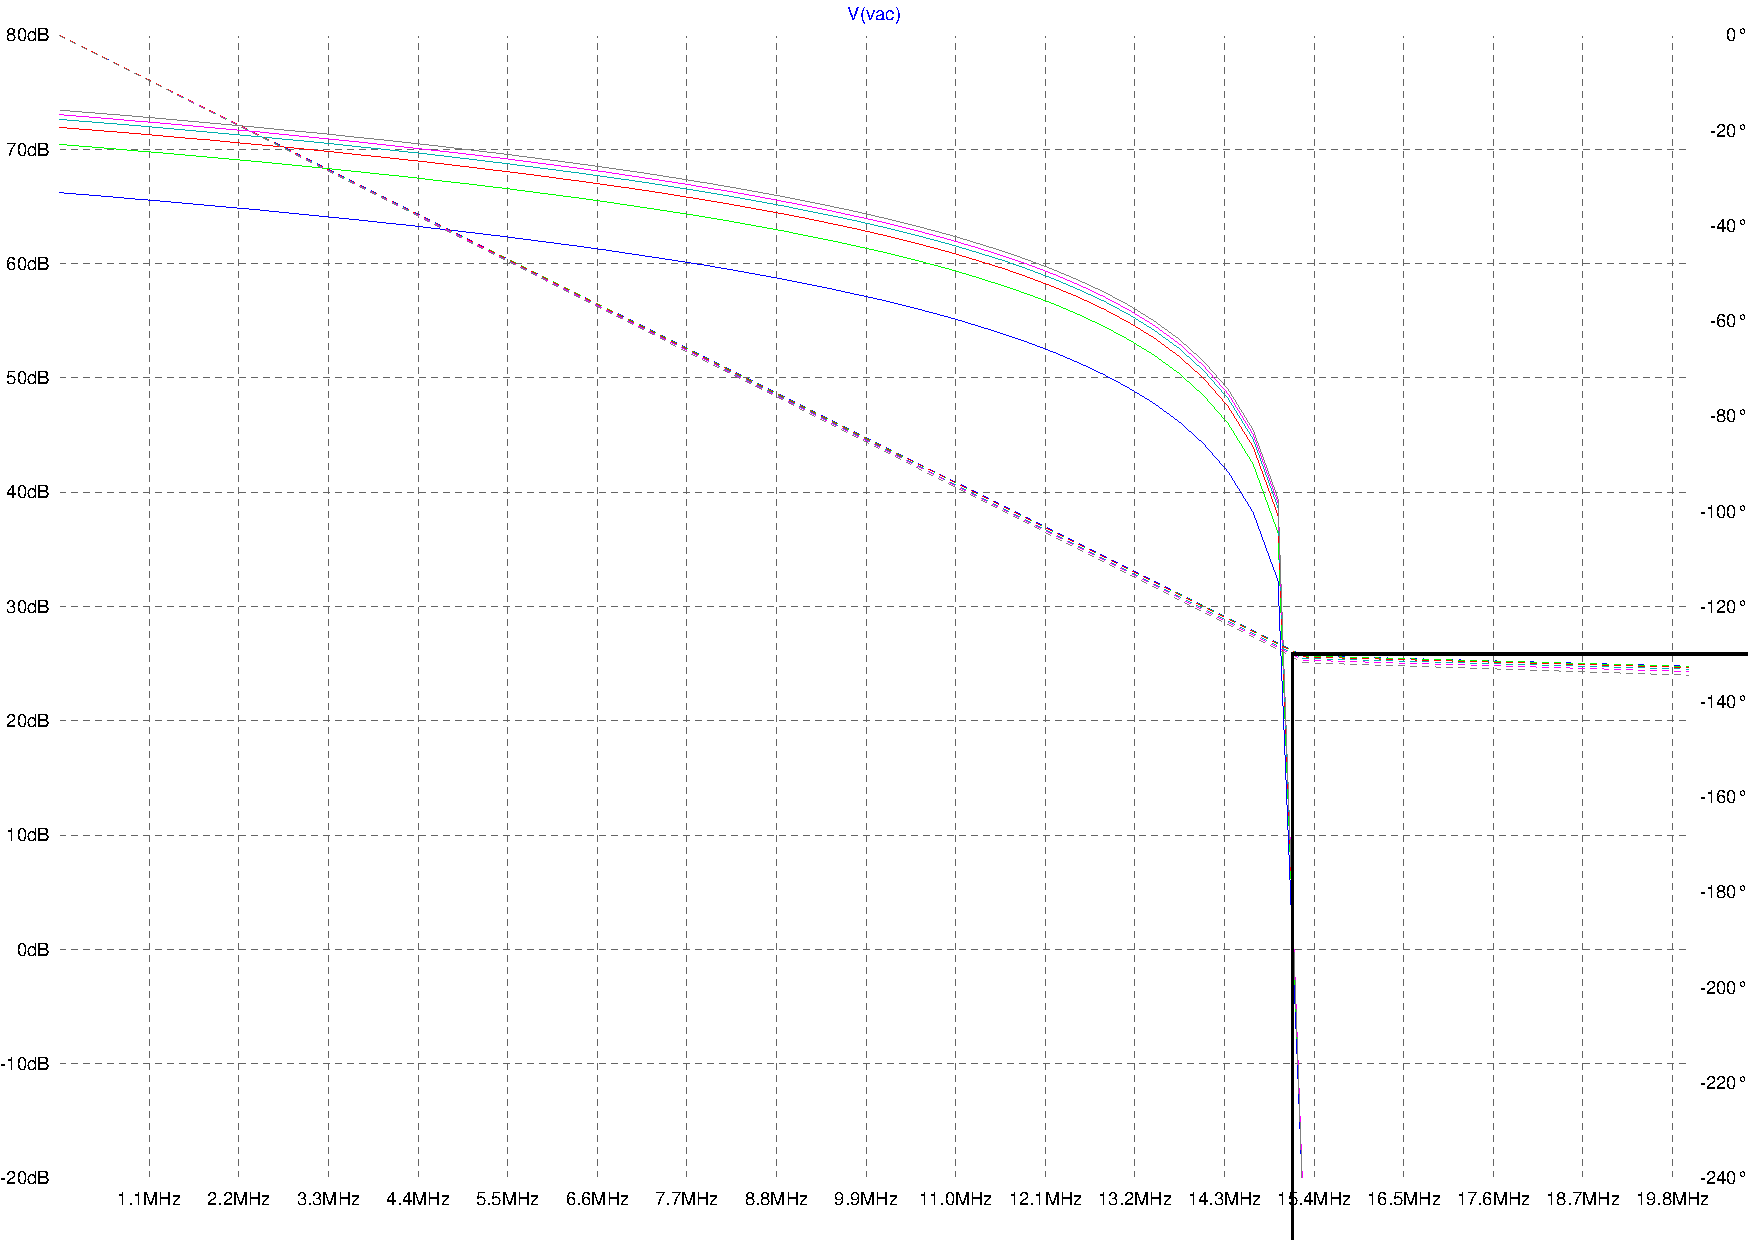
\includegraphics[width=\textwidth]{./images/BasicAC-multi.pdf}
	\caption{The gain and phase of the device for common mode levels $0.3V$, $0.4V$, $0.5V$, $0.6V$, $0.7V$, and $0.8V$}
	\label{fig:Sac}
\end{figure}

Figure \ref{fig:Sac1K} is interesting shows the gain increase from $0dB$ to about $36dB$.
This is rather unexpected behaviour as the gain would normally be expected to be high at DC and then fall away as the frequency increases.
